\beginsong{Edelweißpiraten}[
    wuw={Herwig Steymans, Hans-Jörg Maucksch}, 
    bo={280}, 
    pfii={70}, 
    pfiii={26}, 
    siru={209}, 
    index={Sie saßen oft am Märchensee},
]

\beginverse
\endverse
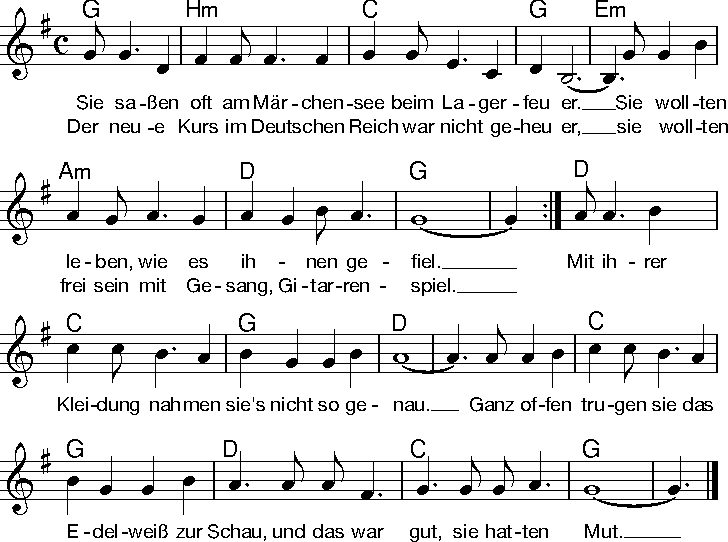
\includegraphics[draft=false, width=1\textwidth]{Noten/Lied032.pdf}	

\beginverse
\[G]Sie hielten \[Hm]nichts von den \[C]braunen Nazi\[G]horden, \[Em]
sie hielten \[Am]nichts von dem Ge\[D]schrei nach Heil und \[G]Sieg.
\[G]Was war denn \[Hm]bloß aus ihrem \[C]Vaterland ge\[G]worden? \[Em]
Man schürte \[Am]offen den ver\[D]brecherischen \[G]Krieg.
\[D]Da gab's nur \[C]eins zu tun: Be\[G]frei'n wir dieses \[D]Land!
\[D]Da durfte \[C]keiner ruh'n, wir \[G]leisten Wider\[D]stand!
Sie hatten \[C]Mut und das war \[G]gut.
\endverse

\beginchorus
\endchorus
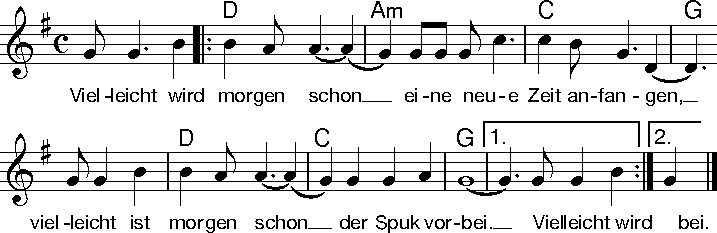
\includegraphics[draft=false, width=1\textwidth]{Noten/Lied032_1.pdf}	

\beginverse
^Da gab's 'nen ^Güterzug mit ^Kriegsgerät und ^Waffen ^
und was man ^sonst noch braucht für ^einen Völker^mord.
^Sie machten ^sich an den ^Gleisen zu ^schaffen, ^
der Zug er^reichte niemals ^den Bestimmungs^ort.
^Und Essens^marken aus dem ^Parteibüro der ^Stadt
^war'n plötzlich ^weg und Zwangsar^beiter wurden ^satt
und das war ^gut, und das war ^gut.
\endverse

\beginverse
^Sie glaubten ^fest daran, dass ^sie den Sieg er^ringen, ^
sie glaubten ^fest daran, aus ^Schaden wird man ^klug.
^Sie glaubten ^fest daran, als ^sie zum Galgen ^gingen, ^
sie glaubten ^fest daran, als ^man sie vorher ^schlug.
^Und dann die ^Angst, die vor ^jeder Folter ^steht,
^die ist so ^groß, dass man den ^besten Freund ^verrät,
versteht man ^gut, versteht man ^gut.
\endverse

\beginverse
^Sie stehen ^heute noch auf ^manchen schwarzen ^Listen, ^
ich würd' fast ^sagen, es ist ^wieder mal so^weit.
^In Amt und ^Würden sitzen ^immer noch Fa^schisten ^
und zum to^talen Krieg ist ^mancher schnell be^reit.
^Doch seh' ich ^Tausende, und ^das beruhigt mich ^sehr,
^die zeigen ^offen das zer^brochene Ge^wehr,
und das macht ^Mut, und das macht ^Mut.
\endverse

\beginchorus
\lrep Und dann wird \[D]morgen schon\[Am] eine neue \[C]Zeit anfangen\[G]
und dann ist \[D]morgen schon\[C] der Spuk vor\[G]bei. \rrep
\endchorus

\endsong

\beginscripture{}
Die Edelweißpiraten waren eine Gruppe Jugendlicher zur Zeit des Dritten Reichs, die sich der Hitlerjugend nicht anschließen wollten. Als sie weiterhin auf Fahrten gingen, wurden sie von der Gestapo verfolgt und wurden oppositionell politisch. Bis zuletzt wurden Edelweißpiraten, die an einem Abzeichen erkennbar waren, verfolgt und erschossen. Bis heute sind sie nicht als Widerstandsgruppe anerkannt. Dieses Lied reflektiert besonders die Bedeutung der Ehrenfelder Gruppe.
\endscripture
